\addcontentsline{toc}{chapter}{Занятие 2. События и операции над ними. Пространство элементарных событий}
\chapter*{Занятие 2. События и операции над ними. Пространство элементарных событий}

\addcontentsline{toc}{section}{Контрольные вопросы и задания}
\section*{Контрольные вопросы и задания}

\subsubsection*{Приведите определение вероятностного эксперимента, вероятностного пространства, случайного события.}

Вероятностным экспериментом называется явление, исход которого для нас не определён, и которое можно повторить любое число раз независимым образом.

Вероятностное пространство --- совокупность всех исходов вероятностного эксперимента, $ \Omega $.

Случайное событие --- подмножество всех исходов вероятностного эксперимента, $ A \subset \Omega $.

\subsubsection*{Запишите основные операции над случайными событиями и дайте их теоретико-множественную интерпретацию.}

Операции будем иллюстрировать на диаграммах Эйлера-Венна.
На рис.\ref{fig:2} заштрихованы области, которые соответствуют событиям, являющимся результатами таких операций.

Пересечением (произведением) двух событий А и В называют событие С, происходящее тогда и только тогда,
когда одновременно происходят оба события А и В, т.е событие,
состоящее из тех и только тех элементарных исходов, которые принадлежат и события А, и событию В (рис.\ref{fig:2}, а).

Пересечение событий А и В записывают следующим образом: $ C = A \cap B $, или $ C = AB $.

События А и В называют несовместимыми, или непересекающимися, если их пересечение является невозможным событием, т.е если $ A \cap B = \emptyset$ (рис.\ref{fig:2}, б).

В противном случае события называют совместимыми, или пересекающимися.

\begin{figure}[h!]
  \centering
  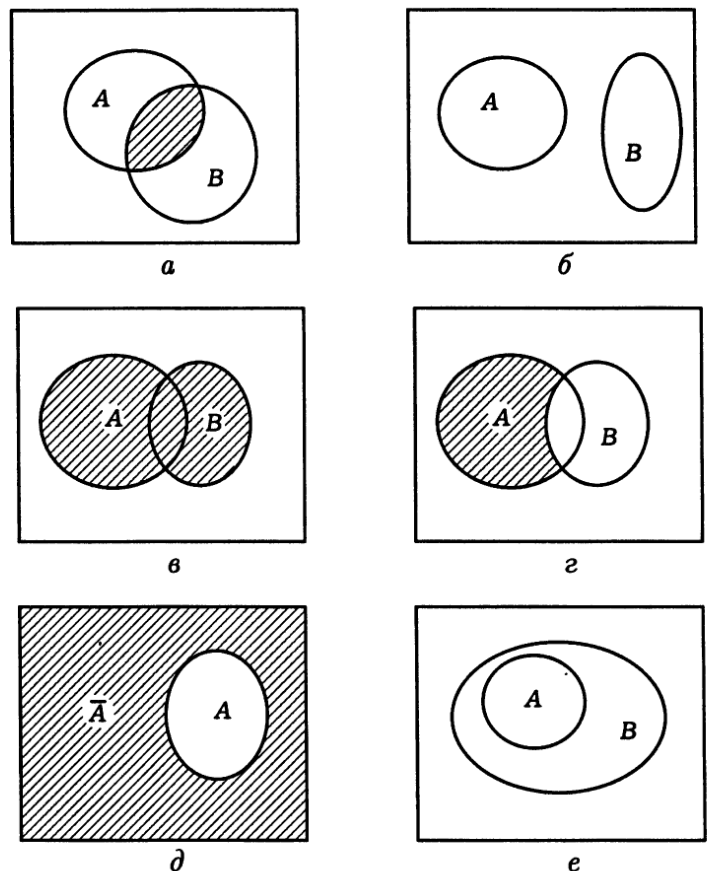
\includegraphics[width=.7\textwidth]{./pictures/2.png}
  \caption{Диаграммы Эйлера-Венна для операций над событиями}
  \label{fig:2}
\end{figure}

Объединением (суммой) двух событий А и В называют событие С,
происходящее тогда и только тогда,
когда происходит хотя бы одно из событий А или В, т.е.
событие С, состоящее из тех элементарных исходов, которые принадлежат хотя бы одному из подмножеств А или В (рис.\ref{fig:2}, в).

Объединение событий А и В записывают в виде $ C = A \cup B $.

Разностью двух событий А и В называют событие С,
происходящее тогда и только тогда,
когда происходит событие А,
но не происходит событие В, т.е. событие С, состоящее из тех элементарных исходов, которые принадлежат А, но не принадлежат В (рис.\ref{fig:2}, г).

Разность событий А и В записывают в виде: $ C = A \setminus B $.

Дополнением события А (обычно обозначают $ \overline{A} $) называют событие, происходящее тогда и только тогда, когда не происходит событие А (рис.\ref{fig:2}, д).
Другими словами, $ \overline{A} = \Omega \setminus A $.

Событие А включено в событие В,
что записывается $ A \subset B $,
если появление события А обязательно влечёт за собой наступление события В (рис.\ref{fig:2}, е),
или каждый элементарный исход $ \omega $, принадлежащий А, обязательно принадлежит и событию В.

Верхний предел последовательности $ \{ A_n : n \geq 1 \} $ --- это случайное событие,
состоящее в том, что произошло бесконечно много событий из исходной последовательности:
$$ \varlimsup \limits_{ n \to \infty } A_n =
\bigcap \limits_{n \geq 1} \bigcup \limits_{ m \geq n } A_m.$$

$ \forall n \exists m \geq n : A_m $ произошло.

Нижний предел последовательности:
$ \{ A_n : n \geq 1 \} $ --- это случайное событие, состоящее в том, что произошли все события, начиная с некоторого из исходной последовательности:
$$ \varliminf \limits_{ n \to \infty } A_n =
\bigcup \limits_{ n = 1 }^\infty \bigcap \limits_{ m = n }^\infty A_m.$$

$ \exists n \forall m \geq n $ происходит событие $A_m$.

\subsubsection*{Сформулируйте законы де Моргана.}

Первый закон де Моргана гласит: <<Если неверно, что есть и первое, и второе, то неверно либо одно из, либо оба>>, что выражается следующей формулой:
$ \overline{ AB } = \overline{ A } \cup \overline{ B }$.

Второй закон де Моргана гласит: <<Если неверно, что есть первое, или неверно, что есть второе, то неверно, что есть первое и второе>>, что выражается следующей формулой:
$ \overline{ A \cup B} = \overline{ A }$ $ \overline{ B }$.

Законы де Моргана верны для любого конечного числа событий:
\begin{equation*}
\begin{split}
\overline{ A_1 \cup A_2 \cup \dotsc \cup A_n } =
\overline{ A_1 } \, \overline{ A_2 } \, \dotsc \overline{ A_n }, \\
\overline{ A_1 A_2 \dotsc A_n } =
\overline{ A_1 } \cup \overline{ A_2 } \cup \dotsc \cup \overline{ A_n }.
\end{split}
\end{equation*}

\addcontentsline{toc}{section}{Аудиторные задачи}
\section*{Аудиторные задачи}

\subsubsection*{2.3}

\textit{Задание.} Рассмотрим эксперимент, который состоит в подбрасывании трёх монет.
Постройте множество $ \Omega $ элементарных событий этого эксперимента.
Опишите событие A, которое состоит в том, что выпало не меньше двух гербов.
Вычислите вероятность события A.

\textit{Решение.} Пусть эксперимент состоит в подбрасывании одной монеты.
При математическом описании этого опыта естественно отвлечься от несущественных возможностей
(например, монета встанет на ребро) и ограничиться только двумя элементарными исходами:
выпадение <<герба>> (обозначим этот исход $ \omega_1 $) и выпадением <<цифры>> (обозначим этот исход $\omega_2$).
Таким образом, $ \Omega_1 = \{ \omega_1, \omega_2 \} $.

При подбрасывании двух монет пространство элементарных исходов будет содержать три элемента,
т.е. $ \Omega_2 = \{ \omega_{11}, \omega_{12}, \omega_{22} \} $, где, например, $\omega_{11}$ --- появление <<герба>> и на первой, и на второй монете.

При подбрасывании трёх монет пространство элементарных исходов будет содержать элементов, т.е.
$ \Omega_3 = \Omega = \{ \omega_{111}, \omega_{112}, \omega_{122}, \omega_{222} \} $, где, например,
$ \omega_{111} $ --- появление <<герба>> и на первой, и на второй, и на третьей монете.

Событие A состоит в том, что выпало не меньше двух гербов, т.е. два или три герба.
Выберем из $ \Omega $ такие исходы: $ A = \{ \omega_{122}, \omega_{222} \} $.

Поскольку $ |A| = 2, | \Omega | = 4$, то
$$ P(A) = \frac{ |A| }{| \Omega |} =
\frac{2}{4} =
\frac{1}{2}.$$

\subsubsection*{2.4}

\textit{Задание.} Пусть A, B, C --- произвольные события.
Найдите выражения для событий, который состоят в том, что из событий A, B и C:
\begin{enumerate}[label=\alph*)]
\item произошло только  A;
\item произошли A и B, но не произошло C;
\item произошли все три события;
\item произошло хотя бы одно из этих событий;
\item произошло хотя бы два события;
\item произошло одно и только одно событие;
\item произошло два и только два события;
\item ни одно из событий не произошло;
\item произошло не больше двух событий.
\end{enumerate}

\textit{Решение.}
\begin{enumerate}[label=\alph*)]
\item $ A \cap \overline{ B } \cap \overline{ C } $;
\item $ A \cap B \cap \overline{ C } $;
\item $ A \cap B \cap C $;
\item $ A \cup B \cup C $;
\item $ \left( A \cap B  \cap \overline{C} \right) \cup \left( A \cap \overline{B} \cap C \right) \cup \left( \overline{A} \cap B \cap C \right) $;
\item $ \left( A \cap \overline{ B } \cap \overline{ C } \right) \cup \left( B \cap \overline{ A } \cap \overline{ C } \right)
\cup \left( C \cap \overline{ A } \cap \overline{ B } \right) $;
\item $ \left( A \cap B \cap \overline{ C } \right) \cup \left( A \cap C \cap \overline{ B } \right) \cup \left( B \cap C \cap \overline{ A } \right) $;
\item $ \overline{ A } \cap \overline{ B } \cap \overline{ C } $;
\item $ \left( \overline{ A } \cap \overline{ B } \cap \overline{ C } \right) \cup
\left( A \cap \overline{ B } \cap \overline{ C } \right) \cup
\left( B \cap \overline{ A } \cap \overline{ C } \right) \cup
\left( C \cap \overline{ A } \cap \overline{ B } \right) \cup
\left( A \cap B \cap \overline{ C } \right) \cup \\
\cup \left( A \cap C \cap \overline{ B } \right) \cup
\left( B \cap C \cap \overline{ A } \right)$.
\end{enumerate}

\subsubsection*{2.5}

\textit{Задание.} Пусть A и B --- некоторые события.
Упростите выражение
$$ C = \overline{ \overline{ A \cap \overline{ B } } \cup \overline{ A \cup B } \cup \left( B \cap A \right) }.$$

\textit{Решение.}
$ C =
\overline{ \overline{ A \cap \overline{ B }}} \cap \overline{ \overline{ A \cup B }} \cap \overline{ B \cap A } =
A \cap \overline{B} \cap \left( A \cup B \right) \cap \left( \overline{B} \cup \overline{A} \right) = \\
= A \cap \left[ \left( \overline{B} \cap A \right) \cup \left( \overline{B} \cap B \right) \right] \cap \left( \overline{B} \cup \overline{A} \right) =
A \cap \overline{B} \cap A \cap \left( \overline{B} \cup \overline{A} \right) =
A \cap \overline{B} \cap \left( \overline{B} \cup \overline{A} \right) = \\
= \left[ \left( A \cap \overline{B} \right) \cup \left( A \cap \overline{A} \right) \right] \cap \overline{B} =
A \cap \overline{B} \cap \overline{B} =
A \cap \overline{B}$.

\subsubsection*{2.6}

\textit{Задание.} Пусть $ \{ A_n, n \in \mathbb{N} \}, \{ B_n, n \in \mathbb{N} \} $ --- некоторые последовательности событий.
Объясните, что значат события $ \varlimsup \limits_{n \to \infty } A_n, \varliminf \limits_{n \to \infty } A_n$.
Докажите, что:
\begin{enumerate}[label=\alph*)]
\item $ \overline{ \varlimsup \limits_{ n \to \infty } A_n } =
\varliminf \limits_{ n \to \infty } \overline{ A_n }$;
\item $ \varlimsup \limits_{ n \to \infty } \left( A_n \cup B_n \right) =
\varlimsup \limits_{ n \to \infty } A_n \cup \varlimsup \limits_{ n \to \infty } B_n $.
\end{enumerate}

\textit{Решение.} Верхний предел последовательности $ \{ A_n : n \geq 1 \} $ ---
это случайное событие, состоящее в том, что произошло бесконечно много событий из исходной последовательности:
$$ \varlimsup \limits_{ n \to \infty } A_n =
\bigcap \limits_{ n \geq 1 } \bigcup \limits_{ m \geq n} A_m.$$

$ \forall n \exists m \geq n : A_m $ произошло.

Нижний предел последовательности:
$ \{ A_n : n \geq 1 \}$ --- это случайное событие, состоящее в том, что произошли все события, начиная с некоторого из исходной последовательности:
$$ \varliminf \limits_{ n \to \infty } A_n =
\bigcup \limits_{ n = 1 }^\infty \bigcap \limits_{ m = n }^\infty A_m.$$

$ \exists n \forall m \geq n $ происходит событие $A_m$.

\begin{enumerate}[label=\alph*)]
\item $\overline{ \varlimsup \limits_{ n \to \infty } A_n } =
\overline{ \bigcap \limits_{ n \geq 1} \bigcup \limits_{ m \geq n} A_m } =
\bigcup \limits_{ n \geq 1} \overline{ \bigcup \limits_{ m \geq n} A_m } =
\bigcup \limits_{ n \geq 1} \bigcap \limits_{ m \geq n} \overline{ A_m } =
\varliminf \limits_{ n \to \infty} \overline{ A_n }$;

\item $\varlimsup \limits_{ n \to \infty } \left( A_n \cup B_n \right) =
\bigcap \limits_{ n \geq 1} \bigcup \limits_{ m \geq n} \left( A_m \cup B_m \right) =
\prod \limits_{ n = 1 }^\infty \sum \limits_{ m = n }^\infty \left( A_m + B_m \right) = \\
= \prod \limits_{ n = 1 }^\infty \sum \limits_{ m = n }^\infty A_m + \prod \limits_{ n = 1 }^\infty \sum \limits_{ m = n }^\infty B_m =
\varlimsup \limits_{ n \to \infty } A_n \cup \varlimsup \limits_{ n \to \infty } B_n $.
\end{enumerate}

\subsubsection*{2.7}

\textit{Задание.} Пусть $ \{ A_n, n \in \mathbb{N} \} $ --- некоторая последовательность событий, $ \mathbbm{1} ( A ) $ --- индикатор события A.
Докажите, что $ \mathbbm{ 1 } \left( \varlimsup \limits_{ n \to \infty } A_n \right) =
\varlimsup \limits_{ n \to \infty } \mathbbm{ 1 } \left( A_n \right) $.

\textit{Решение.} Рассмотрим 4 случая: 

\begin{enumerate}
\item $ \mathbbm{ 1 } \left( \varlimsup \limits_{ n \to \infty } A_n \right) = 0,
\varlimsup \limits_{ n \to \infty } \mathbbm{ 1 } \left( A_n \right) = 0 $;
\item $ \mathbbm{ 1 } \left( \varlimsup \limits_{ n \to \infty } A_n \right) = 0,
\varlimsup \limits_{ n \to \infty } \mathbbm{ 1 } \left( A_n \right) = 1 $;
\item $ \mathbbm{ 1 } \left( \varlimsup \limits_{ n \to \infty } A_n \right) = 1,
\varlimsup \limits_{ n \to \infty } \mathbbm{ 1 } \left( A_n \right) = 0 $;
\item $ \mathbbm{ 1 } \left( \varlimsup \limits_{ n \to \infty } A_n \right) = 1,
\varlimsup \limits_{ n \to \infty } \mathbbm{ 1 } \left( A_n \right) = 1 $.
\end{enumerate}

Нужно доказать, что возможны только первый и последний случаи.

Верхний предел последовательности
$ \{ A_n : n \geq 1 \} $ --- это случайное событие, состоящее в том, что произошло бесконечно много событий из исходной последовательности:
$$ \varlimsup \limits_{ n \to \infty } A_n =
\bigcap \limits_{ n \geq 1} \bigcup \limits_{ m \geq n} A_m.$$

Индикатор --- функция двух переменных:
$ \mathbbm{1} \left( \omega, A \right) $,
где $\omega$ --- элементарный исход (то, что произошло), A --- случайное событие (то, что рассматриваем).
Если $\omega \in A$, то индикатор равен 1, иначе --- 0.

Индикатор верхнего предела равен нулю
$ \left( \mathbbm{ 1 } \left( \varlimsup \limits_{ n \to \infty } A_n \right) = 0 \right)$ --- значит, произошло конечное множество событий из $A_n$.
Значит, с какого-то момента события перестали происходить, и предел индикаторов равен нулю: $ \varlimsup \limits_{ n \to \infty } \mathbbm{ 1 } \left( A_n \right) = 0$.

Если индикатор от верхнего предела равен единице
$$ \left( \mathbbm{ 1 } \left( \varlimsup \limits_{ n \to \infty } A_n \right) =
\mathbbm{ 1 } \left( \bigcap \limits_{ n \geq 1} \bigcup \limits_{ m \geq n } A_m \right) =
1 \right) ,$$
то произошло бесконечное множество событий из $A_n$.
Это значит, во-первых, что пересечение не пустое, а во-вторых, что элементарный исход принадлежит этому пересечению.
Верхний предел последовательности событий --- это такое случайное событие,
что каждый случайный исход из него принадлежит бесконечному количеству событий из последовательности.
Поэтому
$ \varlimsup \limits_{ n \to \infty } \mathbbm{ 1 } \left( A_n \right) = 1 $.

\subsubsection*{2.8}

\textit{Задание.} Пусть B и C --- два события.
Положим $ A_n = B $, если n чётное и $ A_n = C $, если n нечётное.
Найдите событие, которое состоит в том, что:
\begin{enumerate}[label=\alph*)]
\item произошло бесконечно много событий из последовательности $ \{ A_n \}_{ n = 1 }^\infty $;
\item произошло только конечное количество событий из последовательности $ \{ A_n \}_{ n = 1 }^\infty $.
\end{enumerate}

\textit{Решение.}
\begin{enumerate}[label=\alph*)]
\item По определению $ \varlimsup \limits_{ n \to \infty } A_n = \bigcap \limits_{ n \geq 1} \bigcup \limits_{ m \geq n} A_m $.

При $ n = 1: \bigcup \limits_{ m \geq 1} A_m = A_1 \cup A_2 \cup A_3 \cup \dotsc = B \cup C $.
Пересечение бесконечного количества одинаковых множеств даёт $ \varlimsup \limits_{ n \to \infty } A_n = B \cup C $;

\item по определению $ \varliminf \limits_{ n \to \infty } A_n = \bigcup \limits_{ n = 1 }^\infty \bigcap \limits_{ m = n }^\infty A_m = B \cap C $.

При $ n = 1 : \bigcap \limits_{ m \geq 1 } A_m = A_1 \cap A_2 \cap A_3 \cap \dotsc = B \cap C $, поэтому $ \varliminf \limits_{ n \to \infty } A_n = B \cap C $.
\end{enumerate}

\subsubsection*{2.9}

\textit{Задание.} Рассмотрим эксперимент, который состоит в выборе наугад точки в квадрате с вершинами в точках $ A(0, 0), B(0, 1), C(1, 1) $ и $ D(1, 0) $.
Опишите и изобразите вероятностное пространство этого эксперимента и следующие события:
\begin{enumerate}[label=\alph*)]
\item A = {данная точка оказалась на расстоянии не меньшем чем 1/4 от сторон квадрата};
\item B = {данная точка оказалась внутри круга с центром в начале координат и радиусом 1/2};
\item $ \overline{ A }, \overline{ B }, A \cap B $.
\end{enumerate}

\textit{Решение.} Пространство элементарных событий ( \ref{fig:29}, а)) опишем как множество упорядоченных пар
$ \Omega = \{ (x, y), 0 \leq x \geq 1, 0 \leq y \geq 1 \} $, где x --- первая координата точки, y --- вторая координата точки.

\begin{figure}[h!]
  \centering
  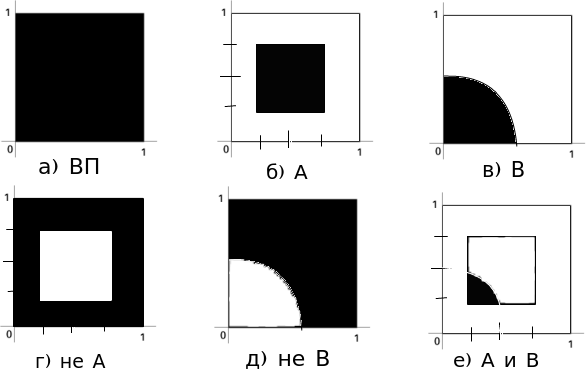
\includegraphics[width=.7\textwidth]{./pictures/2_9.png}
  \caption{Вероятностное пространство и события из задачи 2.9}
  \label{fig:29}
\end{figure}

\begin{enumerate}[label=\alph*)]
\item $ A = \{ (x, y), \frac{3}{4} \leq x \geq \frac{1}{4}, \frac{3}{4} \leq y \geq \frac{1}{4}, \} $ ( \ref{fig:29}, б));

\item $ B = \{ (x, y), x \geq 0, y \geq 0, x^2 + y^2 \leq \frac{1}{2} \} $ ( \ref{fig:29}, в));

\item событие $ \overline{ A } $ означает, что событие A не произошло, то есть расстояние от точки до сторон квадрата оказалось больше 1/4 ( \ref{fig:29}, г)):
$$ \overline{ A } =
\{ (x, y), \frac{3}{4} > x > \frac{1}{4},
\frac{3}{4} > y > \frac{1}{4} \}.$$

Событие $ \overline{ B } $ означает, что данная точка не оказалась внутри круга с центром в начале координат и радиусом 1/2 ( \ref{fig:29}, д)):
$$ \overline{ B } =
\{ (x, y),
\frac{1}{2} > x^2 + y^2 \leq 1,
x \leq 1,
y \leq 1. \} $$

Событие $ A \cap B $ означает, что произошло и событие A, и событие B ( \ref{fig:29}, е)).
Отсюда имеем, что данная точка оказалась на расстоянии не меньшем чем 1/4 от сторон квадрата, а так же внутри круга с центром в начале координат и радиусом 1/2, т.е.
$$ A \cap B =
\{ (x, y),
x \geq \frac{1}{4},
y \geq \frac{1}{4},
x^2 + y^2 \leq \frac{1}{2} \}.$$
\end{enumerate}

\addcontentsline{toc}{section}{Дополнительные задачи}
\section*{Дополнительные задачи}

\subsubsection*{2.10}

\textit{Задание.} Пусть A --- множество из n элементов,
$ A_1,  \dotsc , A_k $ --- подмножества A такие, что ни одно из подмножеств не является частью другого,
а $ i_1,  \dotsc , i_k $ --- количество элементов подмножеств $ A_1,  \dotsc , A_k $ соответственно.
Докажите, что
$$ \sum \limits_{ r = 1 }^k \frac{ 1 }{ C_n^{ i_r } } \leq 1.$$

\textit{Решение.} Умножим слева и справа на произведение знаменателей:
$$ \prod \limits_{r=1}^k C_n^{i_r} \sum \limits_{r=1}^k \frac{1}{C_n^{i_r}} \leq
\prod \limits_{r=1}^k C_n^{i_r}. $$

Внесём произведение под знак суммы:
$$ \sum \limits_{r=1}^k \frac{ \prod \limits_{r'=1}^k C_n^{i_{r'}}}{C_n^{i_r}} \leq
\prod \limits_{r=1}^k C_n^{i_r}. $$

Упростим:
$$ \sum \limits_{r=1}^k \prod \limits_{1 \leq r' \leq k}^{r' \neq r} C_n^{i_{r'}} \leq
\prod \limits_{r=1}^k C_n^{i_r}. $$

Обозначим номер наибольшего слагаемого как r:
$$r =
arg \max \limits_{1 \leq r \leq k} \prod \limits_{1 \leq r' \leq k}^{r' \neq r} C_n^{i_{r'}}.$$

Сумма слагаемых не больше чем наибольшее из них взятое k раз, т.е.
$$ \sum \limits_{r=1}^k \prod \limits_{1 \leq r' \leq k}^{r' \neq r} C_n^{i_{r'}} \leq
k \cdot \prod \limits_{1 \leq r' \leq k}^{r' \neq m} C_n^{i_{r'}} \leq
\prod \limits_{r=1}^k C_n^{i_r}. $$

Поделим правую и левую часть полученного неравенства на произведение, стоящее в левой части:
$$ k \leq
\frac{ \prod \limits_{r=1}^k C_n^{i_r}}{ \prod \limits_{1 \leq r' \leq k}^{r' \neq m} C_n^{i_{r'}}} =
C_n^m. $$

Если $ k \leq n $, то неравенство выполняется для любого возможного m кроме $ m = 0 $ и $ m = n $.

$ m = 0 $ возможно только если $A_1$ --- пустое множество и $k = 1$,
потому что если бы там были другие множества, пустое было бы их подмножеством, что противоречит условию задачи.
Тогда $ C_0^0 = 1 \leq 1$.

$ m = n $, то $ A_1 = A, k = 1 $, значит $C_n^n = 1$.
Если будут другие подмножества кроме $A_1$, то они будут подмножествами $A_1$, что противоречит условию.

\paragraph*{Формулы Стирлинга.}

Распишем левую часть неравенства:
$$ \sum \limits_{r=1}^k \frac{1}{C_n^{i_r}} =
\sum \limits_{r=1}^k \frac{1}{ \frac{n!}{i_{r}! \left(n-i_r\right)!} } =
\sum \limits_{r=1}^k \frac{i_{r}! \left(n-i_r\right)!}{n!}.$$

Получили неравенство:
$$\sum \limits_{r=1}^k \frac{i_{r}! \left(n-i_r\right)!}{n!} \leq 1.$$

Умножим левую и правую части неравенства на $n!$.
Левая часть:
$$ n! \cdot \sum \limits_{r=1}^k \frac{i_{r}! \left(n-i_r\right)!}{n!} =
\sum \limits_{r=1}^k i_{r}! \left(n-i_r\right)!.$$

Получили неравенство:
$$\sum \limits_{r=1}^k i_{r}! \left(n-i_r\right)! \leq n!. $$
Нижний и верхний пределы для факториала:
$$ \sqrt{2 \pi n} \left( \frac{n}{e} \right)^n \exp \left( \frac{1}{12 n+1} \right) <
n! <
\sqrt{2 \pi n} \left( \frac{n}{e} \right)^n \exp \left( \frac{1}{12 n} \right). $$

Возьмём для левой части неравенства верхний предел, а для правой --- нижний:
\begin{equation*}
\begin{split}
\sum \limits_{r=1}^k \sqrt{2 \pi i_r} \left( \frac{i_r}{e} \right)^{i_r} \exp \left( \frac{1}{12 i_r} \right)
\left( \frac{i_r}{e} \right)^{i_r} \sqrt{2 \pi  \left( n-i_r\right) }
\left( \frac{n-i_r}{e} \right)^{n-i_r} \times \\
\times \exp \left( \frac{1}{12 \left( n-i_r\right) } \right) \leq 
\sqrt{2 \pi n} \left( \frac{n}{e} \right)^n \exp \left( \frac{1}{12 n+1} \right).
\end{split}
\end{equation*}

Сократим на $ \sqrt{2 \pi } $ и упростим:
\begin{equation*}
\begin{split}
\sum \limits_{r=1}^k \sqrt{i_r \left( n-i_r \right) }
\exp \left( \frac{1}{12 i_r} + \frac{1}{12 \left( n-i_r \right) } \right) \left( \frac{i_r}{e} \right)^{i_r}
\left( \frac{n-i_r}{e} \right)^{n-i_r} \leq \\
\leq \sqrt{n} \left( \frac{n}{e} \right)^n \exp \left( \frac{1}{12 n+1} \right).
\end{split}
\end{equation*}

Упростим экспоненты в знаменателях левой части:
$$ \exp \left( - i_r \right) \exp \left( i_r - n \right) =
\exp \left( - i_r + i_r - n \right) =
\exp \left( -n \right).$$

В правой части имеем такую же степень экспоненты, поэтому сократим:
\begin{equation*}
\begin{split}
\sum \limits_{r=1}^k \sqrt{i_r \left( n-i_r \right) }
\exp \left( \frac{1}{12 i_r} + \frac{1}{12 \left( n-i_r \right) } \right) i_r^{i_r} \left( n-i_r \right)^{n-i_r} \leq \\
\leq \sqrt{n} n^n \exp \left( \frac{1}{12 n+1} \right).
\end{split}
\end{equation*}

Приведём подобные:
$$ \sum \limits_{r=1}^k i_r^{i_r + \frac{1}{2} } \left( n-i_r \right)^{n - i_r + \frac{1}{2} }
\exp \left( \frac{1}{12 i_r} + \frac{1}{12 \left( n-i_r \right) } \right) \leq
n^{n + \frac{1}{2} } \exp \left( \frac{1}{12 n+1} \right). $$

Приведём к общему знаменателю дроби в степени экспоненты в левой части:
$$ \frac{1}{12 i_r} + \frac{1}{12 \left( n-i_r \right) } =
\frac{n - i_r + i_r}{12 i_r \left( n-i_r \right) } =
\frac{n}{12 i_r \left( n-i_r \right) }. $$

Подставим в неравенство:
$$ \sum \limits_{r=1}^k i_r^{i_r + \frac{1}{2} } \left( n-i_r \right)^{n - i_r + \frac{1}{2} }
\exp \left( \frac{n}{12 i_r \left( n-i_r \right) } \right) \leq 
n^{n + \frac{1}{2} } \exp \left( \frac{1}{12 n+1} \right). $$

Упростим выражение в левой части так, что оно станет больше:
\begin{equation*}
\begin{split}
\sum \limits_{r=1}^k i_r^{i_r + \frac{1}{2} } n^{n - i_r + \frac{1}{2} }
\exp \left( \frac{n}{12 i_r \left( n-i_r \right) } \right) \leq \\
\leq n^{n + \frac{1}{2} } \exp \left( \frac{1}{12 n+1} \right).
\end{split}
\end{equation*}

Сократим на $ n^{n + \frac{1}{2} } $.
Получим:
$$ \sum \limits_{r=1}^k i_r^{i_r + \frac{1}{2} } \left( \frac{1}{n} \right)^{i_r}
\exp \left( \frac{n}{12 i_r \left( n-i_r \right) } \right) \leq
\exp \left( \frac{1}{12 n+1} \right). $$

Внесём $ i_r^{i_r} $ в числитель дроби и поделим на экспоненту из правой части:
$$ \sum \limits_{r=1}^k \sqrt{i_r} \left( \frac{i_r}{n} \right)^{i_r}
\exp \left( \frac{n}{12 i_r \left( n-i_r\right) } - \frac{1}{12 n + 1} \right) \leq 1. $$

Сведём дроби в степени экспоненты к общему знаменателю:
\begin{equation*}
\begin{split}
\frac{n}{12 i_r \left( n-i_r \right) } - \frac{1}{12 n + 1} =
\frac{n \left( 12 n + 1 \right) - 12 i_r \left( n-i_r \right) }{12 i_r \left( n-i_r \right) \left( 12 n + 1\right) } = \\
= \frac{12 n^2 + n - 12 i_r n + 12 i_r^2}{12 i_r \left( n-i_r \right) \left( 12 n + 1\right) } =
\frac{12 n^2 + n - 12 i_r n + 12 i_r^2}{ \left( 12 i_r n - 12 i_r^2 \right) \left( 12 n + 1 \right) } = \\
= \frac{12 n^2 + n - 12 i_r n + 12 i_r^2}{144 n^2 i_r + 12 i_r n - 144 i_r^2 n - 12 i_r^2} =
\frac{12 \left( n^2 -2 i_r n + i_r^2 \right) + n + 12 i_r n}{144 n^2 i_r + 12 i_r n - 144 i_r^2 n - 12 i_r^2} = \\
= \frac{12 \left( n-i_r\right)^2 + n + 12 i_r n }{144 n^2 i_r + 12 i_r n - 144 i_r^2 n - 12 i_r^2}.
\end{split}
\end{equation*}

Упростим выражение, используя нижний предел для количества сочетаний:
$$ \left( \frac{n}{k} \right)^k \leq C_n^k. $$

Получим:
$$\sum \limits_{r=1}^k \frac{1}{C_n^{i_r}} \leq
\sum \limits_{r=1}^k \frac{1}{\left( \frac{n}{i_r} \right)^{i_r}} =
\sum \limits_{r=1}^k \left( \frac{i_r}{n} \right)^{i_r}. $$

\addcontentsline{toc}{section}{Домашнее задание}
\section*{Домашнее задание}

\subsubsection*{2.11}

\textit{Задание.} Рассмотрим эксперимент, который состоит в подбрасывании трёх игральных кубиков.
Опишите множество $ \Omega $ элементарных событий этого эксперимента; из скольки элементарных событий оно состоит?
Опишите событие С, которое состоит в том, что на всех кубиках выпало одинаковое количество очков.
Вычислите вероятность события С.

\textit{Решение.} Пространство элементарных событий опишем как множество упорядоченных троек
$ \Omega = \{ \left( i, j, k \right),
i = \overline{ 1, 6 },
j = \overline{ 1, 6 },
k = \overline{ 1, 6 } \} $,
где i --- количество очков, которые выпали на первом кубике,
j --- количество очков, которые выпали на втором кубике,
k --- количество очков, которые выпали на третьем кубике.

Можем рассматривать тройку чисел как вектор длины 3.
Первой компонентой вектора может быть любое значение из $ \{ 1, 2, 3, 4, 5, 6 \} $.
Его можно выбрать $ C_6^1 = 6 $ способами.
Таким же образом находим, что есть 6 способов выбрать вторую компоненту вектора и 6 --- третью.
По правилу умножения имеем $ 6 \cdot 6 \cdot 6 = 6^3 = 216 $ разных векторов указанного вида, или элементарных событий.

$ C = \{ (1, 1, 1), (2, 2, 2), (3, 3, 3), (4, 4, 4), (5, 5, 5), (6, 6, 6) \} $.
Поскольку
$$ |C| = 6,
|\Omega| = 216, $$
то
$$ P(C) =
\frac{ |C| }{ |\Omega| } =
\frac{ 6 }{ 216 } =
\frac{ 1 }{ 36 }.$$

\subsubsection*{2.12}

\textit{Задание.} Монету подбрасывают до тех пор, пока она не выпадет 2 раза подряд одной и той же стороной, но не больше четырёх раз.
Опишите множество $ \Omega $ элементарных событий.
Опишите следующие события и вычислите их вероятности:
\begin{enumerate}[label=\alph*)]
\item А = { эксперимент закончился на втором подбрасывании};
\item В = { эксперимент закончился на третьем подбрасывании};
\item C = { эксперимент закончился на четвёртом подбрасывании}.
\end{enumerate}

\textit{Решение.}  Пусть опыт состоит в однократном подбрасывании монеты.
При математическом описании этого опыта естественно отвлечься от несущественных возможностей
(например, монета встанет на ребро) и ограничиться только двумя элементарными исходами:
выпадение <<герба>> (обозначим этот исход $ \omega_1 $) и выпадением <<цифры>> (обозначим этот исход $ \omega_2 $).
Таким образом, $ \Omega_1 = \{ \omega_1, \omega_2 \} $.

При двукратном подбрасывании монеты пространство элементарных исходов будет содержать четыре элемента, т.е.
$$ \Omega_2 = \{ \omega_{11}, \omega_{12}, \omega_{21}, \omega_{22} \},$$
где, например, $ \omega_{11} $ --- появление <<герба>> и при первом, и при втором подбрасываниях.
В данном случае эксперимент может завершиться, если при двукратном подбрасывании монеты она выпала два раза одной и той же стороной.
Поэтому $ A = \{ \omega_{11}, \omega_{22} \} $.

При трёхкратном подбрасывании монеты пространство элементарных исходов будет содержать 8 элементов, т.е.
$$ \Omega_3 =
\{ \omega_{111}, \omega_{112}, \omega_{122}, \omega_{121}, \omega_{211}, \omega_{221}, \omega_{212}, \omega_{222} \},$$
где, например, $ \omega_{111} $ --- появление <<герба>> и при первом, и при втором, и при третьем подбрасываниях.
Исходом эксперимента могут быть такие 3 подбрасывания, при которых в первый раз выпала одна сторона монеты, а в следующие 2 --- другая, т.е.
$ B = \{ \omega_{122}, \omega_{211} \} $.

При четырёхкратном подбрасывании монеты пространство исходов будет содержать 16 элементов, т.е
\begin{equation*}
\begin{split}
\Omega_4 =
\{ \omega_{1111}, \omega_{1112}, \omega_{1121}, \omega_{1211}, \omega_{2111}, \omega_{1122}, \omega_{1212}, \omega_{2112}, \omega_{2211}, \omega_{2121}, \omega_{1221}, \\
\omega_{1222}, \omega_{2122}, \omega_{2212}, \omega_{2221}, \omega_{2222}\},
\end{split}
\end{equation*}
где, например, $ \omega_{1111} $ --- появление <<герба>> при всех четырёх подбрасываниях.
Чтобы эксперимент не закончился раньше четвёртого подбрасывания, уберём из множества
$ \Omega_4 $ такие его элементы, которые обеспечивают конец эксперимента при втором и третьем подбрасывании.
Получим $ C = \{ \omega_{1211}, \omega_{1212}, \omega_{2121}, \omega_{2122} \} $.

Пространство элементарных исходов состоит из всех элементов множеств A, B и C, т.е.
$$ \Omega =
\{ \omega_{11}, \omega_{22}, \omega_{122}, \omega_{211}, \omega_{1211}, \omega_{1212}, \omega_{2121}, \omega_{2122} \}.$$

Поскольку $ |A| = 2 $, $ |\Omega| = 8 $, то
$$ P(A) =
\frac{ |A| }{ |\Omega| } =
\frac{2}{8} =
\frac{1}{4}.$$

Так же и $ |B| = 2 $, $ |\Omega| = 8 $, поэтому
$$ P(B) =
\frac{ |B| }{ |\Omega| } =
\frac{2}{8} =
\frac{1}{4}.$$

Поскольку $ |C| = 4 $, $ |\Omega| = 8 $, то
$$ P(C) =
\frac{ |C| }{ |\Omega| } =
\frac{4}{8} =
\frac{1}{2}.$$

\subsubsection*{2.13}

\textit{Задание.} Рабочий произвёл n деталей.
Пусть событие $ A_i $ состоит в том, что i-я деталь имеет дефект.
Запишите событие, которое состоит в том, что:
\begin{enumerate}[label=\alph*)]
\item ни одна из деталей не имеет дефектов;
\item хотя бы одна из деталей имеет дефект;
\item ровно одна деталь имеет дефект;
\item ровно две детали имеют дефект;
\item хотя бы две детали не имеют дефектов;
\item не больше двух деталей имеют дефект.
\end{enumerate}

\textit{Решение.}
\begin{enumerate}[label=\alph*)]
\item $ \overline{A_1} \cap \overline{A_2} \cap \dotsc \cap \overline{A_n} =
\bigcap \limits_{i=1}^n \overline{A_i}$;

\item $ A_1 \cup A_2 \cup \dotsc \cup A_n =
\bigcup \limits_{i=1}^n A_i $;

\item $ \bigcup \limits_{i=1}^n \left( A_i \cap \left( \bigcap \limits_{j=1}^n \overline{A_j} \right) \right), \, j \neq i$;

\item $ \bigcup \limits_{i, j=1}^n \left( A_i \cap A_j \cap \left( \bigcap \limits_{k=1}^n \overline{A_k} \right) \right), \, i \neq j \neq k$;

\item $D =$ \{хотя бы две детали не имеют дефектов\} = \{иди две детали не имеют дефектов, или 3 детали не имеют дефектов, ..., или $n$ деталей не имеет дефектов\}.

Рассмотрим противоположное событие: $ \overline{D} =$ \{меньше двух деталей не имеют дефекта\} = \{все детали с дефектами\} $ \cup $
\{ровно одна деталь не имеет дефекта\} $= \left( \bigcap \limits_{i=1}^n A_i \right) \cup \left( \bigcup \limits_k \overline{A_k} \bigcap \limits_{i \neq k} A_i \right) $.

Вернёмся к нужному событию.
Воспользуемся правилом де Моргана:
$D =
\overline{ \left( \bigcap \limits_{i=1}^n A_i \right) \cup \left( \bigcup \limits_k \overline{A_k} \bigcap \limits_{i \neq k} A_i \right) }$; 

\item $E =$ \{не больше двух деталей имеют дефект\} = \{все детали без дефектов\} $ \cup $ \{одна деталь с дефектом\} $ \cup
$ \{две детали с дефектом\}
$= \left( \bigcap \limits_{i=1}^n \overline{A_i} \right) \cup
\left( \bigcup \limits_{j=1}^n A_j \cap \left( \bigcap \limits_{k=1}^n \overline{A_k} \right) \right) \cup
\left( \bigcup \limits_{l,m=1}^n \left( A_l \cap A_m \cap \left( \bigcap \limits_{t=1}^n \overline{A_t} \right) \right) \right), \, i \neq \\
\neq j \neq k \neq l \neq m \neq t$.
\end{enumerate}

\subsubsection*{2.14}

\textit{Задание.} Пусть А, В, С --- некоторые события.
Что означают равенства:
\begin{enumerate}[label=\alph*)]
\item $ A \cap B \cap C = A $?
\item $ A \cup B \cup C = A $?
\end{enumerate}

\textit{Решение.}
\begin{enumerate}[label=\alph*)]
\item Событие А содержится и в событии В, и в событии С;

\item событие А содержит и событие В, и событие С.
\end{enumerate}

\subsubsection*{2.15}

\textit{Задание.} Упростите выражение:
\begin{enumerate}[label=\alph*)]
\item $ \left( A \cup B \right) \cup \left( A \cup \overline{ B } \right) $;
\item $ \left( A \cup B \right) \cap \left( \overline{ A } \cup B \right) \cap \left( A \cup \overline{ B } \right) $.
\end{enumerate}

\textit{Решение.} Используя свойства операций над событиями, получаем:
\begin{enumerate}[label=\alph*)]
\item $ \left( A \cup B \right) \cup \left( A \cup \overline{ B } \right) =
A \cup B \cup A \cup \overline{ B } =
A \cup A \cup B \cup \overline{ B } =
\left( A \cup A \right) \cup \left( B \cup \overline{ B } \right) = \\
= A \cup \Omega =
\Omega $;

\item $ \left( A \cup B \right) \cap \left( \overline{ A } \cup B \right) \cap \left( A \cup \overline{ B } \right) =
\left( A \cup B \right) \cap \left( A \cup \overline{ B } \right) \cap \left( \overline{ A } \cup B \right) = \\
= \left( A \cup \left( B \cap \overline{ B } \right) \right) \cap \left( \overline{ A } \cup B \right) =
\left( A \cup \emptyset \right) \cap \left( \overline{ A } \cup B \right) =
A \cap \left( \overline{ A } \cup B \right) = \\
= \left( A \cap \overline{ A } \right) \cup \left( A \cap B \right) =
\emptyset \cup \left( A \cap B \right) =
A \cap B $.
\end{enumerate}

\subsubsection*{2.16}

\textit{Задание.} Пусть $ \{ A_n, n \in \mathbb{ N } \}, \{ B_n, n \in \mathbb{ N } \}$ --- некоторые последовательности событий.
Докажите, что:
\begin{enumerate}[label=\alph*)]
\item $ \overline{ \varliminf \limits_{ n \to \infty } A_n } =
\varlimsup \limits_{ n \to \infty } \overline{ A_n }$;

\item $ \varlimsup \limits_{ n \to \infty } A_n \cap \varliminf \limits_{ n \to \infty } B_n \subseteq
\varlimsup \limits_{ n \to \infty } \left( A_n \cap B_n \right) \subseteq
\varlimsup \limits_{ n \to \infty } A_n \cap \varlimsup \limits_{ n \to \infty } B_n $.
\end{enumerate}

\textit{Решение.}
\begin{enumerate}[label=\alph*)]
\item $ \overline{ \varliminf \limits_{ n \to \infty } A_n } =
\overline{ \bigcup \limits_{ n \geq 1 } \bigcap \limits_{ m \geq n } A_n } =
\bigcap \limits_{ n \geq 1 } \overline{ \bigcap \limits_{ m \geq n } A_n } =
\bigcap \limits_{ n \geq 1 } \bigcup \limits_{ m \geq 1 } \overline{ A_m } =
\varlimsup \limits_{ n \to \infty } \overline{ A_n }$;

\item докажем, что нижний предел входит в верхний.
Распишем нижний предел:

$ \varliminf \limits_{ n \to \infty } B_n =
\bigcup \limits_{ n = 1 }^\infty \bigcap \limits_{ m = n }^\infty B_m =
\left( B_1 \cap B_2 \cap \dotsc \right) \cup \left( B_2 \cap B_3 \cap \dotsc \right) \cup \dotsc = \\
= B_1 B_2 B_3 \dotsc + B_2 B_3 B_4 \dotsc + \dotsc $.

Распишем верхний предел:

$ \varlimsup \limits_{ n \to \infty } B_n =
\bigcap \limits_{ n = 1 }^\infty \bigcup \limits_{ m = n }^\infty B_m =
\left( B_1 \cup B_2 \cup \dotsc \right) \cap \left( B_2 \cup B_3 \cup \dotsc \right) \cap \dotsc = \\
= \left( B_1 + B_2 + B_3 + \dotsc \right) \left( B_2 + B_3 + B_4 + \dotsc \right) \dotsc = \\
= B_1 B_2 \dotsc + B_2 B_3 \dotsc + B_3 B_4 \dotsc + \dotsc + B_1 B_3 \dotsc + B_1 B_4 \dotsc + B_2 B_3 \dotsc + \dotsc = \\
= \varliminf \limits_{ n \to \infty } B_n + B_1 B_3 \dotsc + B_1 B_4 \dotsc + B_2 B_3 \dotsc + \dotsc $

Видим, что в верхний предел, помимо нижнего, входят дополнительные члены.
Поэтому нижний предел входит в верхний, т.е.
$$ \varliminf \limits_{ n \to \infty } B_n \subseteq
\varlimsup \limits_{ n \to \infty } B_n.$$

Значит первое выражение входит в третье:
$$ \varlimsup \limits_{ n \to \infty } A_n \cap \varliminf \limits_{ n \to \infty } B_n \subseteq
\varlimsup \limits_{ n \to \infty } A_n \cap \varlimsup \limits_{ n \to \infty } B_n.$$

Докажем, что второе выражение входит в третье.
Распишем второе выражение:

$ \varlimsup \limits_{ n \to \infty } \left( A_n \cap B_n \right) =
\bigcap \limits_{ n \geq 1 } \bigcup \limits_{ m \geq n } \left( A_m \cap B_m \right) =
\bigcap \limits_{ n \geq 1 } \bigcup \limits_{ m \geq n } C = \\
= \left( C_1 \cup C_2 \cup \dotsc \right) \cap \left( C_2 \cup C_3 \cup \dotsc \right) \cap \dotsc = \\
= \left( \left( A_1 \cap B_1 \right) \cup \left( A_2 \cap B_2 \right) \cup \dotsc \right) \cap
\left( \left( A_2 \cap B_2 \right) \cup \left( A_3 \cap B_3 \right) \cup \dotsc \right)\cap \dotsc = \\
= \left( A_1 B_1 + A_2 B_2 + \dotsc \right) \left( A_2 B_2 + A_3 B_3 + \dotsc \right) \dotsc$

Распишем третье выражение:

$ \varlimsup \limits_{ n \to \infty } A_n \cap
\varlimsup \limits_{ n \to \infty } B_n =
\left( \bigcap \limits_{ n \geq 1 } \bigcup \limits_{ m \geq n } A_m \right)
\cap \left( \bigcap \limits_{ n \geq 1 } \bigcup \limits_{ m \geq n } B_m \right) = \\
= \left( \prod \limits_{ n = 1 }^\infty \sum \limits_{ m = n }^\infty A_m \right)
\left( \prod \limits_{ n = 1 }^\infty \sum \limits_{ m = n }^\infty B_m \right) =
\left( A_1 + A_2 + \dotsc \right) \left( A_2 + A_3 + \dotsc \right) \dotsc
\left( \prod \limits_{ n = 1 }^\infty \sum \limits_{ m = n }^\infty B_m \right) = \\
= \left( A_1 \cdot \prod \limits_{ n = 1 }^\infty \sum \limits_{ m = n }^\infty B_m +
A_2 \cdot \prod \limits_{ n = 1 }^\infty \sum \limits_{ m = n }^\infty B_m + \dotsc \right)
\left( A_2 + A_3 + \dotsc \right) \dotsc = \\
= \left[ A_1 \left( B_1 + B_2 + \dotsc \right)
\left( B_2 + B_3 + \dotsc \right) \dotsc \right] +
\left[ A_2 \left( B_1 + B_2 + \dotsc \right)
\left( B_2 + B_3 + \dotsc \right) \dotsc \right] \times \\
\times \left( A_2 + A_3 + \dotsc \right) \dotsc =
\left( \left( A_1 B_1 + A_1 B_2 + \dotsc \right) \left( B_2 + B_3 + \dotsc \right) \dotsc \right) + \\
+ \left( \left( A_2 B_1 + A_2 B_2 + \dotsc \right) \left( B_2 + B_3 + \dotsc \right) \dotsc \right)
\left( A_2 + A_3 + \dotsc \right) \dotsc $

Все члены, полученные во втором выражении, входят в третье, значит
$$ \varlimsup \limits_{ n \to \infty } \left( A_n \cap B_n \right) \subseteq
\varlimsup \limits_{ n \to \infty} A_n \cap
\varlimsup \limits_{ n \to \infty } B_n.$$

Докажем, что первое выражение входит во второе.
Распишем первое выражение:

\begin{equation*}
\begin{split}
\varlimsup \limits_{ n \to \infty } A_n \cap \varliminf \limits_{ n \to \infty } B_n =
\left( \bigcap \limits_{ n \geq 1 } \bigcup \limits_{ m \geq n } A_m \right) \cap
\left( \bigcup \limits_{ n = 1 }^\infty \bigcap \limits_{ m = n }^\infty B_m \right) = \\
= \left( \bigcap \limits_{ n \geq 1 } \bigcup \limits_{ m \geq n } A_m \right) \cap C =
\left( A_1 \cup A_2 \cup \dotsc \right) \cap \left( A_2 \cup A_3 \cup \dotsc \right) \cap \dotsc \cap C = \\
= \left( \left( A_1 \cap C \right) \cup \left( A_2 \cap C \right) \cup \dotsc \right) \cap
\left( A_2 \cup A_3 \cup \dotsc \right) \cap \left( A_3 \cup A_4 \cup \dotsc \right) \cap \dotsc = \\
= \left( A_1 \cdot C + A_2 \cdot C + \dotsc \right) \left( A_2 + A_3 + \dotsc \right)
\left( A_3 + A_4 + \dotsc \right) \dotsc = \\
= \left( A_1 \cdot \sum \limits_{ n = 1 }^\infty \prod \limits_{ m = n }^\infty B_m +
A_2 \cdot \sum \limits_{ n = 1 }^\infty \prod \limits_{ m = n }^\infty B_m + \dotsc \right)
\left( A_2 + A_3 + \dotsc \right) \left( A_3 + A_4 + \dotsc \right) \dotsc =  \\
= \left\{ \left[ A_1 \left( B_1 B_2 \dotsc +B_2 B_3 \dotsc + \dotsc \right) \right] +
\left[ A_2 \left( B_1 B_2 \dotsc +B_2 B_3 \dotsc + \dotsc \right) \right] + \dotsc \right\} \times \\
\times \left( A_2 + A_3 + \dotsc \right) \left( A_3+A_4+ \dotsc \right) \dotsc = \\
= \left( A_1 B_1 B_2 \dotsc + A_1 B_2 B_3 \dotsc + A_2 B_1 B_2 \dotsc + A_2 B_2 B_3 \dotsc + \dotsc \right) \times \\
\times \left( A_2 + A_3 + \dotsc \right) \left( A_3 + A_4 + \dotsc \right) \dotsc = \\
= ( A_2 A_2 B_1 B_2 \dotsc + A_1 A_3 B_1 B_2 \dotsc + A_1 A_2 B_1 B_2 \dotsc + \\
+ A_1 A_3 B_1 B_2 \dotsc + A_2 A_2 B_2 B_3 \dotsc + A_2 A_3 B_2 B_3 \dotsc + \dotsc )
\left( A_3 + A_4+ \dotsc \right) \dotsc = \\
= A_2 A_2 A_3 \dotsc B_1 B_2 \dotsc + A_2 A_2 A_4 \dotsc B_1 B_2 \dotsc + A_1 A_3 A_3 \dotsc B_1 B_2 \dotsc + \\
+ A_1 A_3 A_4 \dotsc B_1 B_2 \dotsc + A_1 A_2 A_3 \dotsc B_1 B_2 \dotsc + A_1 A_2 A_4 \dotsc B_1 B_2 \dotsc + \\
+ A_1 A_3 A_3 \dotsc B_1 B_2 \dotsc + A_1 A_3 A_4 \dotsc B_1 B_2 \dotsc + A_2 A_2 A_3 \dotsc B_2 B_3 \dotsc + \\
+ A_2 A_2 A_4 \dotsc B_2 B_3 \dotsc + A_2 A_3 A_3 \dotsc B_2 B_3 \dotsc + A_2 A_3 A_4 \dotsc B_2 B_3 \dotsc + \dotsc 
\end{split}
\end{equation*}

Вспомним второе выражение:
\begin{equation*}
\begin{split}
\varlimsup \limits_{ n \to \infty } \left( A_n \cap B_n \right) =
\left( A_1 B_1 + A_2 B_2 + A_3 B_3 + \dotsc \right) \left( A_2 B_2 + A_3 B_3 + A_4 B_4 + \dotsc \right) \times \\
\times \left(A_3 B_3 + A_4 B_4 + \dotsc \right) \dotsc = \\
= ( A_1 A_2 B_1 B_2 + A_1 A_3 B_1 B_3 + A_1 A_4 B_1 B_4 + A_2 A_2 B_2 B_2 + A_2 A_3 B_2 B_3 + A_2 A_3 B_2 B_4 + \\
+ A_3 A_2 B_3 B_2 + A_3 A_3 B_3 B_3 + A_3 A_4 B_3 B_4 + \dotsc) \left(A_3 B_3 + A_4 B_4 + \dotsc  \right) \dotsc = \\
= A_1 A_2 A_3 \dotsc B_1 B_2 B_3 \dotsc + A_1 A_2 A_4 \dotsc B_1 B_2 B_4 \dotsc + A_1 A_3 A_3 \dotsc B_1 B_3 B_3 \dotsc + \\
+ A_1 A_3 A_4 \dotsc B_1 B_3 B_4 \dotsc + A_1 A_4 A_3 \dotsc B_1 B_4 B_3 \dotsc + A_1 A_4 A_4 \dotsc B_1 B_3 B_4 \dotsc + \\
+ A_2 A_2 A_3 \dotsc B_2 B_2 B_3 \dotsc + A_2 A_2 A_4 \dotsc B_2 B_2 B_4 \dotsc + A_2 A_3 A_3 \dotsc B_2 B_3 B_3 \dotsc + \\
+ A_2 A_3 A_4 \dotsc B_2 B_3 B_4 \dotsc + A_3 A_2 A_3 \dotsc B_3 B_2 B_3 \dotsc + A_3 A_2 A_4 \dotsc B_3 B_2 B_4 \dotsc + \\
+ A_3 A_3 A_3 \dotsc B_3 B_3 B_3 \dotsc + A_3 A_3 A_4 \dotsc B_3 B_3 B_4 \dotsc + A_3 A_4 A_3 \dotsc B_3 B_4 B_3 \dotsc + \\
+ A_3 A_4 A_4 \dotsc B_3 B_4 B_4 \dotsc + \dotsc
\end{split}
\end{equation*}

Как доказать, что первое выражение входит во второе, не знаю. Поэтому рассмотрим второй метод. Распишем первое выражение через другое определение пределов.

\begin{equation*}
\begin{split}
x \in \varlimsup \limits_{ n \to \infty } \cap \varliminf \limits_{n \to \infty } B_n \Rightarrow
\begin{cases}
x \in \varlimsup \limits_{ n \to \infty } A_n \\
x \in \varliminf \limits_{n \to \infty } B_n
\end{cases}
\Rightarrow
\begin{cases}
\forall n \exists m \geq n : x \in A_m \\
\exists n \forall m \geq n : x \in B_m
\end{cases}
\Rightarrow \\
\Rightarrow \forall n \exists m \geq n : x \in A_m \cap B_m \Rightarrow
x \in \varlimsup \limits_{n \to \infty } \left( A_n \cap B_n \right) \Rightarrow
\begin{cases}
\forall n \exists m \geq n : x \in A_m \\
\forall n \exists m \geq n : x \in B_m
\end{cases}
\Rightarrow \\
\Rightarrow
\begin{cases}
x \in \varlimsup \limits_{n \to \infty } A_n \\
x \in \varlimsup \limits_{n \to \infty } B_n
\end{cases}
\Rightarrow
x \in \varlimsup \limits_{n \to \infty } A_n \cap \varlimsup \limits_{n \to \infty } B_n.
\end{split}
\end{equation*}

Получили требуемый результат.

\subsubsection*{2.17}

\textit{Задание.} Пусть $ \{ A_n , n \in \mathbb{N} \} $ --- некоторая последовательность событий,
$ \mathbbm{1} ( A ) $ --- индикатор события А.
Докажите, что:
$ \mathbbm{1} \left( \varliminf \limits_{n\to\infty} A_n \right) = \varliminf \limits_{n\to\infty} \mathbbm{1} \left( A_n \right) $.

\textit{Решение.} Рассмотрим 4 случая:
\begin{enumerate}
\item $\mathbbm{1}\left(\varliminf\limits_{n\to\infty}A_n\right)=0, \varliminf\limits_{n\to\infty}\mathbbm{1}\left(A_n\right)=0$;
\item $\mathbbm{1}\left(\varliminf\limits_{n\to\infty}A_n\right)=0, \varliminf\limits_{n\to\infty}\mathbbm{1}\left(A_n\right)=1$;
\item $\mathbbm{1}\left(\varliminf\limits_{n\to\infty}A_n\right)=1, \varliminf\limits_{n\to\infty}\mathbbm{1}\left(A_n\right)=0$;
\item $\mathbbm{1}\left(\varliminf\limits_{n\to\infty}A_n\right)=1, \varliminf\limits_{n\to\infty}\mathbbm{1}\left(A_n\right)=1$.
\end{enumerate}

Нужно доказать, что возможны только первый и последний случаи.

Нижний предел последовательности:
$\{ A_n : n \geq 1 \}$ --- это случайное событие, состоящее в том, что произошли все события, начиная с некоторого из исходной последовательности:
$$\varliminf \limits_{n\to\infty} A_n = \bigcup \limits_{n=1}^\infty \bigcap \limits_{m=n}^\infty A_m. $$

Если индикатор нижнего предела равен нулю:
$$ \mathbbm{1} \left( \varliminf \limits_{n\to\infty} A_n \right) = 0 , $$
то нет такого момента, начиная с которого начали происходить все события.
Имеем события, которые произошли, и которые не произошли.
Индикатор событий, которые произошли, равен единице, а которые не произошли --- нулю.
Нижний предел последовательности чисел --- это точная нижняя грань.
Точная нижняя грань последовательности из нулей и единиц равна нулю, т.е.
$$\varliminf \limits_{n\to\infty} \mathbbm{1} \left( A_n \right) = 0 . $$

Если индикатор от нижнего предела равен единице:
$$ \mathbbm{1} \left( \varliminf \limits_{n\to\infty} A_n \right) = 1 , $$
то произошло бесконечное множество событий из $A_n$ начиная с какого-то момента.
Значит индикатор событий начиная с этого момента равен единице.
Поэтому нижний предел равен единице:
$$\varliminf \limits_{n\to\infty} \mathbbm{1} \left( A_n \right) = 1 . $$
\end{enumerate}

\subsubsection*{2.18}

\textit{Задание.} Рассмотрим эксперимент, который состоит в выборе наугад точки в круге единичного радиуса с центром в начале координат.
Опишите и изобразите пространство элементарных событий этого эксперимента, а также следующие события:
\begin{enumerate}[label=\alph*)]
\item A = {произведение координат точки не превышает 1/8};
\item B = {данная точка оказалась внутри круга с центром в начале координат и радиусом 1/4};
\item $ \overline{ A },
\overline{ B },
A \cap B $.
\end{enumerate}

\textit{Решение.}
Пространство элементарных событий опишем как множество упорядоченных пар
$ \Omega =
\{ (x, y), x^2 + y^2 \leq 1 \} $,
где x --- первая координата точки, y --- вторая координата точки (\ref{fig:218}, а)).

\begin{figure}[h!]
  \centering
  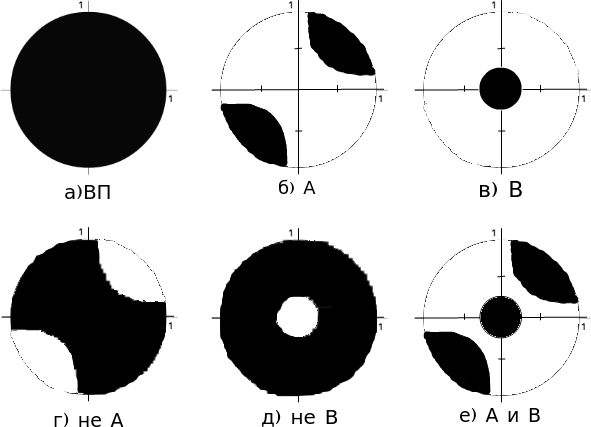
\includegraphics[width=.7\textwidth]{./pictures/2_18.png}
  \caption{Вероятностное пространство и события из задачи 2.18}
  \label{fig:218}
\end{figure}

\begin{enumerate}[label=\alph*)]
\item $ A =
\{ (x, y), x^2 + y^2 \leq 1, xy \leq \frac{ 1 }{ 8 } \} $ (\ref{fig:218}, г));

\item $ B =
\{ (x, y), x^2 + y^2 \leq \frac{ 1 }{ 4 } \} $ (\ref{fig:218}, в));

\item событие $ \overline{ A } $ означает, что событие А не произошло,то есть произведение координат точки превышает 1/8 (\ref{fig:218}, б)):
$$ \overline{ A } =
\{ (x, y), xy > 1/8, x^2 + y^2 \leq 1 \}.$$

Событие $ \overline{ B } $ означает, что точка не оказалась внутри круга радиуса 1/4 (\ref{fig:218}, д)):
$$ \overline{ B } =
\{ (x, y), 1 \geq x^2 + y^2 > \frac{ 1 }{ 4 } \}.$$

Событие $ A \cap B $ означает, что произошло и событие A, и событие B.
Отсюда имеем, что произведение координат точки не должно превышать 1/8, а сумма квадратов координат должна быть не больше 1/4 (\ref{fig:218}, е)), т.е.
$$ A \cap B =
\{ (x, y), x^2 + y^2 \leq \frac{ 1 }{ 4 }, xy \leq \frac{ 1 }{ 8 } \}.$$
\end{enumerate}
